%%%%%%%%%%%%%%%%%%%%%%%%%%%%%%%%%%%%%%%%%%%%%%%%%%%%%%%%%%%%%%%%%%%%%
%
%  This is a sample LaTeX input file for your contribution to 
%  the M&C2019 topical meeting.
%
%  Please use it as a template for your full paper 
%    Accompanying/related file(s) include: 
%       1. Document class/format file: mandc.cls
%       2. Sample Postscript Figure:   figure.pdf
%       3. A PDF file showing the desired appearance: mandc2019_template.pdf
%       4. cites.sty and citesort.sty that might be needed by some users 
%    Direct questions about these files to: palmert@engr.orst.edu
%											mark.dehart@inl.gov
%
%    Notes: 
%      (1) You can use the "dvips" utility to convert .dvi 
%          files to PostScript.  Then, use either Acrobat 
%          Distiller or "ps2pdf" to convert to PDF format. 
%      (2) Different versions of LaTeX have been observed to 
%          shift the page down, causing improper margins.
%          If this occurs, adjust the "topmargin" value in the
%          physor2018.cls file to achieve the proper margins. 
%
%%%%%%%%%%%%%%%%%%%%%%%%%%%%%%%%%%%%%%%%%%%%%%%%%%%%%%%%%%%%%%%%%%%%%


%%%%%%%%%%%%%%%%%%%%%%%%%%%%%%%%%%%%%%%%%%%%%%%%%%%%%%%%%%%%%%%%%%%%%
\documentclass[letterpaper]{mandc2019}
%
%  various packages that you may wish to activate for usage 
\usepackage{tabls}
\usepackage{cites}
\usepackage{epsf}
\usepackage{appendix}
\usepackage{ragged2e}
\usepackage[top=1in, bottom=1.in, left=1.in, right=1.in]{geometry}
\usepackage{enumitem}
\setlist[itemize]{leftmargin=*}
\usepackage{caption}
\captionsetup{width=1.0\textwidth,font={bf,normalsize},skip=0.3cm,within=none,justification=centering}
\usepackage{float}

\newcommand{\tcr}[1]{\textcolor{red}{#1}}
\newcommand{\vr}{\vec{r}}
\newcommand{\vo}{\vec{\Omega}}

%\usepackage[justification=centering]{caption}

%
% Define title...
%
\title{APPROACHES TO LOAD BALANCING \\
MASSIVELY PARALLEL TRANSPORT SWEEPS\\
ON UNSTRUCTURED GRIDS}
%
% ...and authors
%
\author{%
  % FIRST AUTHORS 
  %
  \textbf{Tarek Habib Ghaddar$^1$, Jean C. Ragusa$^1$, Jan Vermaak$^1$, Marvin L. Adams$^1$} \\
$^1$Dept. of Nuclear Engineering, Texas  A\&M University \\
  College Station, TX, 77843-3133 \\ 
     \\
  \url{tghaddar@tamu.edu}, \url{jean.ragusa@tamu.edu}, \url{janv@tamu.edu}, \url{mladams@tamu.edu}
}
%
% Insert authors' names and short version of title in lines below
%
\newcommand{\authorHead}      % Author's names here use et al. if more than 3
           {First author}  
\newcommand{\shortTitle}      % Short title here (Shorten to fit all into a single line)
           {Paper Title }  
%%%%%%%%%%%%%%%%%%%%%%%%%%%%%%%%%%%%%%%%%%%%%%%%%%%%%%%%%%%%%%%%%%%%%
%
%   BEGIN DOCUMENT
%
%%%%%%%%%%%%%%%%%%%%%%%%%%%%%%%%%%%%%%%%%%%%%%%%%%%%%%%%%%%%%%%%%%%%%
\begin{document}
\maketitle
\justify 

\begin{abstract}
  Use 8.5$\times$11 paper size, with 1'' margins on all sides.  A required 200-250 
  word abstract starts on this line.  Leave two blank lines before ``ABSTRACT''
  and one after.  Use 11 point Times New Roman here and single 
  spacing. The abstract is a very brief summary highlighting main 
  accomplishments, what is new, and how it relates to the state-of-the-art.
\end{abstract}
\keywords{list of three to five key words}

\section{INTRODUCTION} 
The steady-state neutron transport equation describes the behavior of neutrons in a medium and is given by Eq. (\ref{continuous transport}):
\begin{multline}
\vo \cdot \vec \nabla \psi(\vr,E,\vo) + \Sigma_t(\vr,E) \psi(\vr,E,\vo)  = \\ 
\int_{0}^{\infty}dE' \int_{4\pi}d\Omega' \Sigma_s(\vr,E'\to E, \Omega'\to\Omega)\psi(\vr,E',\vo')  + S_{ext}(\vr,E,\vo) ,
\label{continuous transport}
\end{multline}
where $\vec{\Omega}\cdot \vec\nabla\psi$ is the leakage term and $\Sigma_t\psi$ is the total collision term (absorption, outscatter, and within group scattering). These represent the loss terms of the neutron transport equation. The right hand side of Eq.~\eqref{continuous transport} represents the gain terms, where $S_{ext}$ is the external source of neutrons and $\int_{0}^{\infty}dE'\int_{4\pi}d\Omega'\Sigma_s(E'\to E, \Omega'\to\Omega)\psi(\vr,E',\vo')$ is the inscatter term, which represents all neutrons scattering from energy $E'$ and direction $\vo'$ into $dE$ about energy $E$ and $d\Omega$ about direction $\vo$. 

Eq. (\ref{angle}) is obtained by assuming isotropic scattering, discretizing in energy, and discretizing in angle using the discrete ordinates method\cite{discrete ordinates}:
\begin{equation}
\vo_m \cdot \vec \nabla \psi_{g,m}(\vr) +\Sigma_{t,g}(\vr) \psi_{g,m}(\vr)  = \frac{1}{4\pi}\sum_{g^{\prime}}\Sigma_{s,g^{\prime}\to g}(\vr)\phi_{g^{\prime}}(\vr) + S_{ext,g,m}(\vr).
\label{angle}
\end{equation}

This allows us to solve a sequence of transport equations for one group and direction at a time. The discrete form of the transport equation is solved via source iteration, described in Eq. (\ref{source iteration}):
\begin{equation}
\vo_m \cdot \vec\nabla \psi_m^{(l+1)}(\vr) + \Sigma_t \psi_m^{(l+1)}(\vr) = q_m^{(l)}(\vr),
\label{source iteration}
\end{equation}
where the gain terms terms have been combined into one general source term, $q_m$. The angular flux of iteration $(l+1)$ is calculated using the $(l^{th})$ value of the scalar flux. 

After the angular and energy dependence have been accounted for, Eq. (\ref{source iteration}) must be discretized in space as well. This is done by meshing the domain and utilizing one of three popular discretization techniques: finite difference\cite{fd}, finite volume\cite{fd}, or discontinuous finite element\cite{Reed}, allowing one cell at a time to be solved. The solution across a cell interface is connected based on an upwind approach, where face outflow radiation becomes face inflow radiation for the downwind cells. 

PDT, Texas A\&M's massively parallel deterministic transport code, employs the transport sweep with the process described above, using a finite element mesh and solving the discrete ordinates form of the transport equation using a discontinuous finite element approach and source iteration\cite{mpadams15, mpadams13}. Initially, PDT only swept on structured, logically Cartesian meshes. As the need to solve problems with more complex geometries arose, PDT added a support for arbitrary polyhedral unstructured meshes. However, this introduced imbalanced partitions, causing runtimes of problems to become unmanageable.

To combat imbalanced partitions, two load balancing algorithms were implemented, referred to in this paper as the original load balancing algorithm and the load balancing by dimension algorithm.


\section{LOAD BALANCING UNSTRUCTURED MESHES IN PDT} 
\label{sec:first}

Before detailing the two load balancing algorithms PDT employs, a quick review of partitioning unstructured meshes in PDT is necessary:
\vspace{-2cm}
\begin{itemize}\itemsep 1pt \parskip 0pt \parsep 0pt
\item ``Cut lines" in 2D (cut planes for 3D) are used to slice through the mesh in the $x$, $y$, and $z$ dimensions.
\item The cut planes form brick partitions, called subsets, that have unstructured meshes inside of them. 
\item The subsets are distributed amongst the processor domain.
\end{itemize}
\vspace{-2cm}
Figure \ref{partioning_example} shows an example of an unstructured mesh partitioned into four subsets.

\begin{figure}[H]
\centering
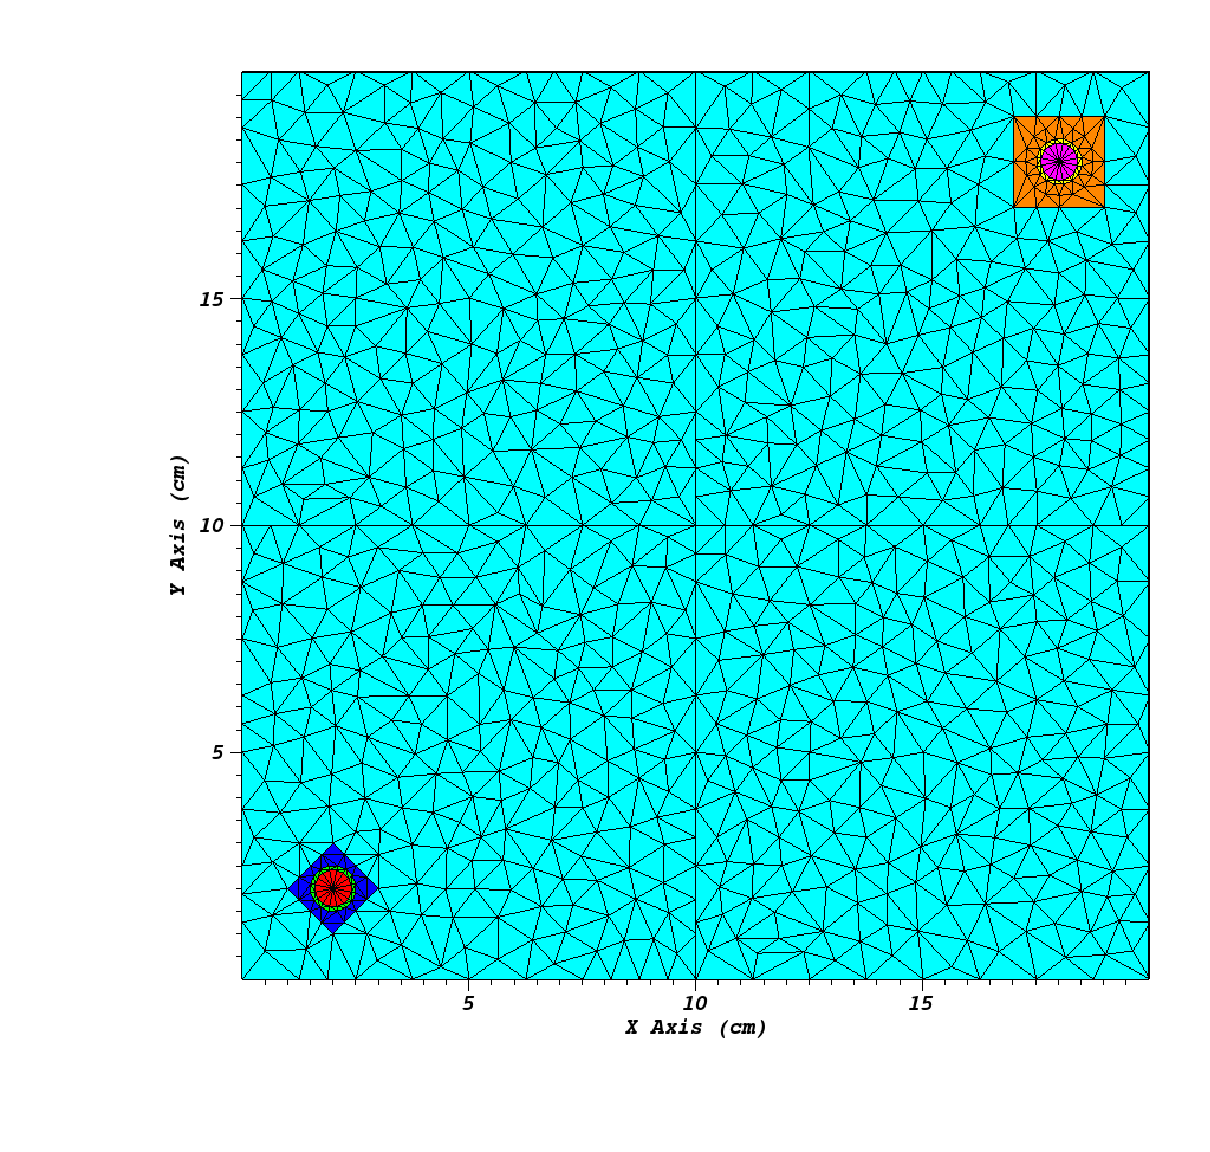
\includegraphics[scale=0.9,trim={0.95in 0.64in 0.35in 0.44in},clip]{Figures/partitioning_example.pdf}
\caption{An unstructured mesh partitioned into four subsets with cut lines at $x,y = 10$ cm.}
\label{partioning_example}
\end{figure}

Both approaches to load balancing move these cut lines in order to redistribute cells more evenly throughout subsets, and therefore processors.

\subsection{Subsection Title: First Character of Each Non-trivial Word is Uppercase} 
\label{sec:second}

Double-space before and after secondary titles is automatic.  Figures and 
tables should appear as close as possible to where they are first
cited, e.g., Fig.~\ref{fig:amdahl}, in the text.  Figures are numbered in Arabic 
numerals, with the caption centered below the figure, in \textbf{boldface}. For a better 
arrangement it is strongly recommended that all the figures must be placed in the``Figures'' 
folder. Triple-space before the figure, and after the figure caption.

\begin{figure}[!htb]
  \centering
  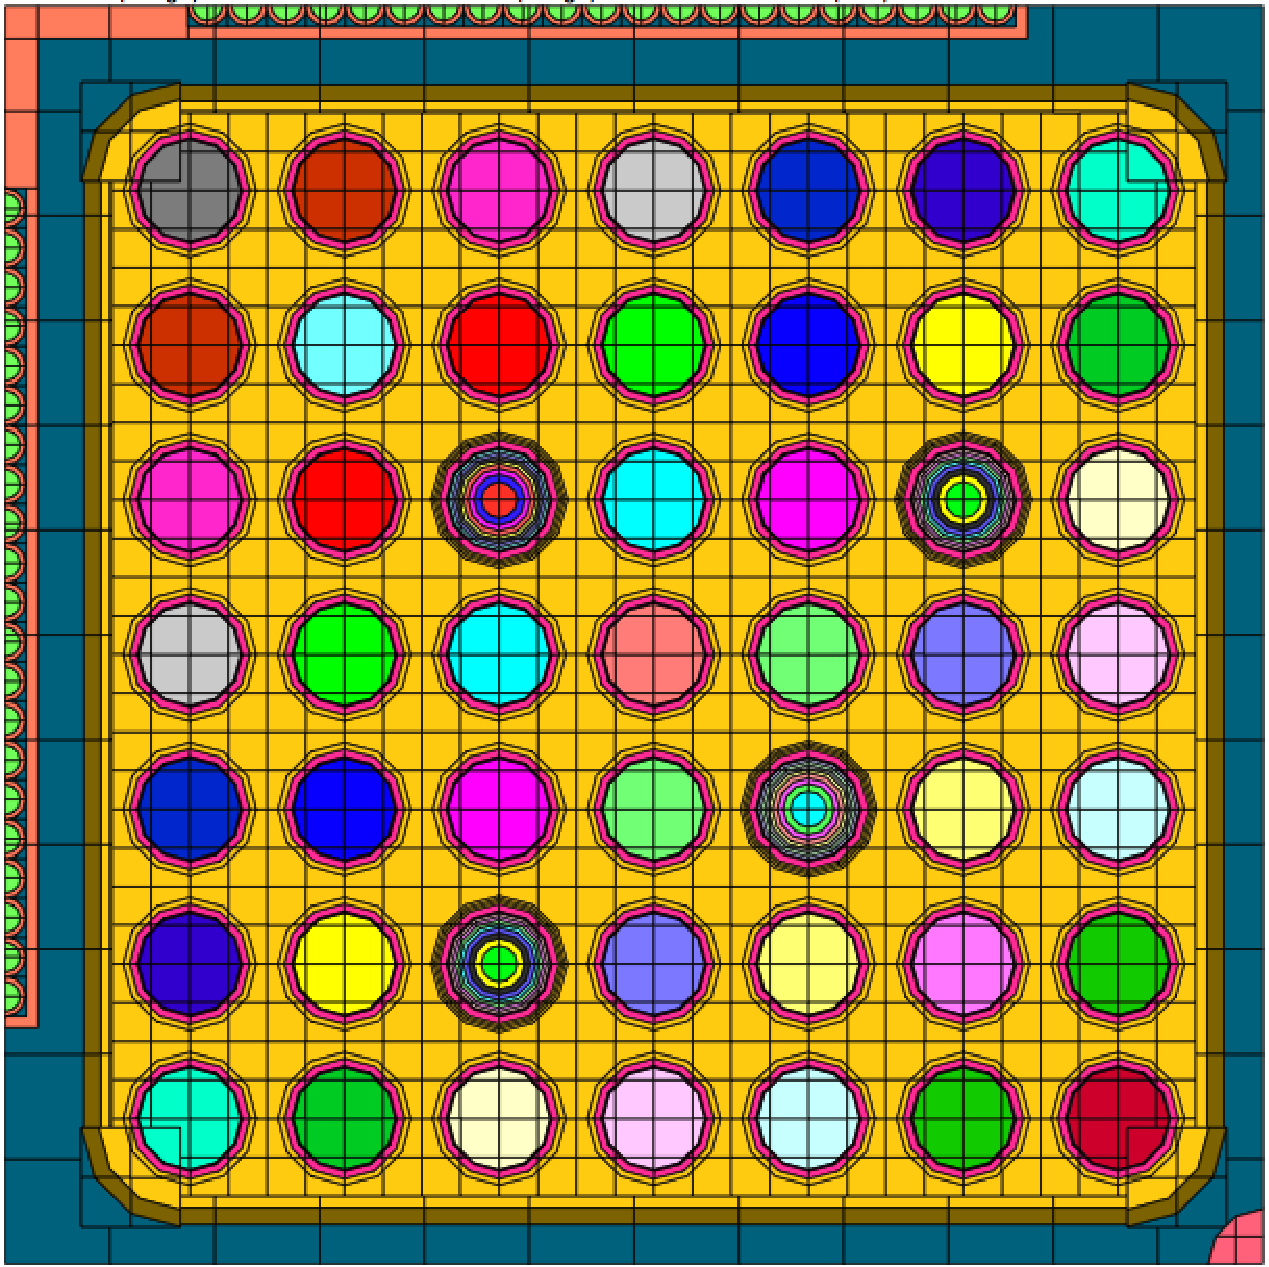
\includegraphics[scale=0.60]{./Figures/figure.pdf}
  \caption{SCALE/TRITON-NEWT Model of BWR Assembly in Order to Show and Example of a Figure and a Multi-line Caption}   
  \label{fig:amdahl}
\end{figure}

When importing figures or any graphical image please verify two things:
\vspace{-0.65cm} % THE DISTANCE BETWEEN THE ":" AND THE FIRST LINE OF THE LIST MAY VARY DEPENDING ON THE TEXT LENGTH, CHANGE THIS VALUE DEPENDING ON YOUR NEEDS.
\begin{itemize} \itemsep1pt \parskip0pt \parsep0pt
\item Any number, text or symbol is in Times font and is not smaller than 
  10-point after reduction to the actual window in your paper
\item That it can be translated into PDF
\end{itemize}

Equations, such as Eq. (\ref{sample_equation}), should be centered and 
sequentially numbered to the flush right of the formula.

\begin{equation}
  \label{sample_equation}
  \mathrm{Speedup}=\frac{1}{\frac{f}{p}+(1-f)}
\end{equation}

The continuation of a paragraph after an equation should not be indented.  
All paragraphs, as well as section or subsection headings, are separated by 
just one single empty line.

\subsubsection{Sub-subsection level and lower: only first character uppercase}

See Table \ref{table:example} for a sample table.  The ``tabls'' package is
recommended for improved row and column spacing.  Notice the caption appears 
above the table by setting the \verb!\caption! command immediately 
after the \verb!\begin{table}!. Tables are numbered in Roman 
numerals, with the caption centered above the table, in \textbf{boldface}.  
Triple-space before and after the table.

\begin{table}[!htb]
  \centering
  \caption{\bf Parallel Performance for the Sample Problem}
  \label{table:example} 
  \begin{tabular}{|c|c|c|c|} \hline 
   Number of & Wall-Clock & Speedup & Efficiency \\
   Processors & Time$^{a}$ (min) & (T$_{s}$/T$_{p}$) & (\%) \\ \hline
    \ 1 &  100.0 & \ ---    & ---  \\ \hline
    \ 2 &   52.6 & \ 1.9    & 95.0 \\ \hline 
  \end{tabular}
\end{table}

\section{CONCLUSIONS}

Present your summary and conclusions here.

\section*{NOMENCLATURE}

If variables are extensively used in the text, a Nomenclature section would be helpful to the readers.

\section*{ACKNOWLEDGEMENTS}

Acknowledge the help of colleagues and sources of funding, as appropriate.

\textbf{As an example:} The format for this template was adapted from the \LaTeX template for the PHYSOR-2018 conference posted and available on the Internet and 
most of the \LaTeX\ format definitions contained in this were already defined. The 
M\&C 2019 organizing committee deeply thank the PHYSOR-2018 technical committee 
for this great support.

% You can enter a bibliography into the document using the following format, or use the 
% bibliography style file "mandc.bst" found in the template directory.  You can use the bibliography style file
% by replacing the current bibliography block with:
% \setlength{\baselineskip}{12pt}
% \bibliographystyle{mandc}
% \bibliography{mandc}

\setlength{\baselineskip}{12pt}
\begin{thebibliography}{300}
\bibitem{journal} B. Author(s), ``Title,'' \emph{Journal Name in Italic}, 
  \textbf{Volume in Bold}, pp. 34-89 (19xx).
\bibitem{proc_paper} C. D. Author(s), ``Article Title,'' \emph{Proceedings of
  Meeting in Italic}, Location, Dates of Meeting, Vol. n, pp. 134-156 
  (19xx).
\bibitem{book} E. F. Author, \emph{Book Title in Italic}, Publisher, City \&
  Country (19xx). 
\bibitem{website} ``Spallation Neutron Source: The next-generation 
  neutron-scattering facility in the United States,'' 
  \url{http://www.sns.gov/documentation/sns\_brochure.pdf} (2002).
\end{thebibliography}

\appendix
\gdef\thesection{APPENDIX \Alph{section}}
\section{Sample Appendix 1}
\label{app:a}
If necessary, include Appendices numbered in upper case alphabetical order. This is \ref{app:a}. 



\end{document}
